\documentclass[12pt]{report}
\usepackage[utf8]{inputenc}
\usepackage[margin=2cm]{geometry}
\usepackage{graphicx}
\usepackage[spanish]{babel}
\usepackage[usenames]{color}

\author{Gisela Villanueva - Raul Marusca\\Coordinador: Juan Gonzalez}
\title{\huge Análisis llamadas telefónicas\\{\Large UNAB - Juzgado Federal de Lomas de Zamora}}

\begin{document}
	\maketitle
	
	\chapter*{Resumen}
	Se requiere identificar un numero telefónico celular (o una lista reducida de números telefónicos) que haya o hayan  operado en las cercanías de una dirección en un determinado periodo de tiempo.\\
	Para ello se dispone de varios reportes entregados por una empresa operadora de redes celulares que tiene cobertura en la zona citada.\\
	Estos reportes cubre una ventana de tiempo mayor a la buscada de manera de encontrar cuales son los números que frecuentan la zona y usar esa información para centrar el estudio en los números poco frecuentes.\\
	\vspace{3mm}\\
	{\Large Importante:} los reportes de la compañía aparentan pertenecer a unas celdas ubicadas en una localidad alejada 20 km del sitio a analizar.\\
	En este reporte consideraremos que esto es una confusión geográfica y que SI los llamados registrados corresponden al sitio correcto.\\
	\vspace{3mm}\\
	A continuación, los detalles:
	
	\chapter*{Análisis}
	\section*{Períodos analizados}
	El hecho ocurrió el día 7 de septiembre de 2023 aproximadamente a las 20:45.\\
	Los reportes suministrados por la compañía de comunicaciones abarcan desde el día 7 de agosto de 2023 a las 0 horas hasta el día 13 de septiembre del mismo año a las 23:59:59.\\
	Se consideran dos posibles \textit{ventanas} de tiempo alrededor del momento del hecho: una de mas-menos 20 minutos (que abarcaría del 7 de septiembre a las 20:25 hasta ese día a las 21:05) y otra de mas-menos 5 minutos (de las 20:40 a las 20:50)
	\section*{Tipos de comunicación}
	El reporte comprende dos tipos de comunicaciones:
	\begin{itemize}
		\item Llamadas SALIENTES\\
		Son las comunicaciones realizadas desde un dispositivo que se halla conectado a la celda reportada.
		\item Llamadas ENTRANTES\\
		
		Son las comunicaciones recibidas por un dispositivo conectado a la celda reportada.
	\end{itemize}
	\section*{Destinos de la comunicación}
	Las comunicaciones pueden ser desde o hacia:
	\begin{itemize}
		\item Una comunicación de datos. 
		\item Un teléfono de la misma compañía. 
		\item Un teléfono de otra compañía.
		\item Un servicio de atención al cliente.
		\item Números gratuitos.
		\item Un teléfono en una provincia argentina.
		\item Un teléfono en otro país.
		\item Un servicio (como WhatsApp Free) que se brinda de forma gratuita.
		\item Un teléfono de línea.
	\end{itemize}
	\section*{Cantidad de llamados}
	En el total del período reportado se realizaron un total de 6.986.719 comunicaciones salientes y 402.632 entrantes.\\
	En la ventana de tiempo de $\pm$ 20 minutos se realizaron 5.893 comunicaciones salientes y 391 entrantes.\\
	En la ventana de tiempo de $\pm$ 5 minutos se realizaron 1.474 comunicaciones salientes y 112 entrantes.\\
	
	En el total del período reportado se contabilizan 69.414 números diferentes realizando comunicaciones salientes. Operando cada uno de ellos entre 1 y 79.226 comunicaciones por dispositivo.\\
	
	En el total del período reportado se contabilizan 36.828 números diferentes realizando comunicaciones entrantes. Recibiendo cada uno de ellos entre 1 y 3856 llamados por dispositivo.\\
	
	\begin{figure}[h]
		\centering
		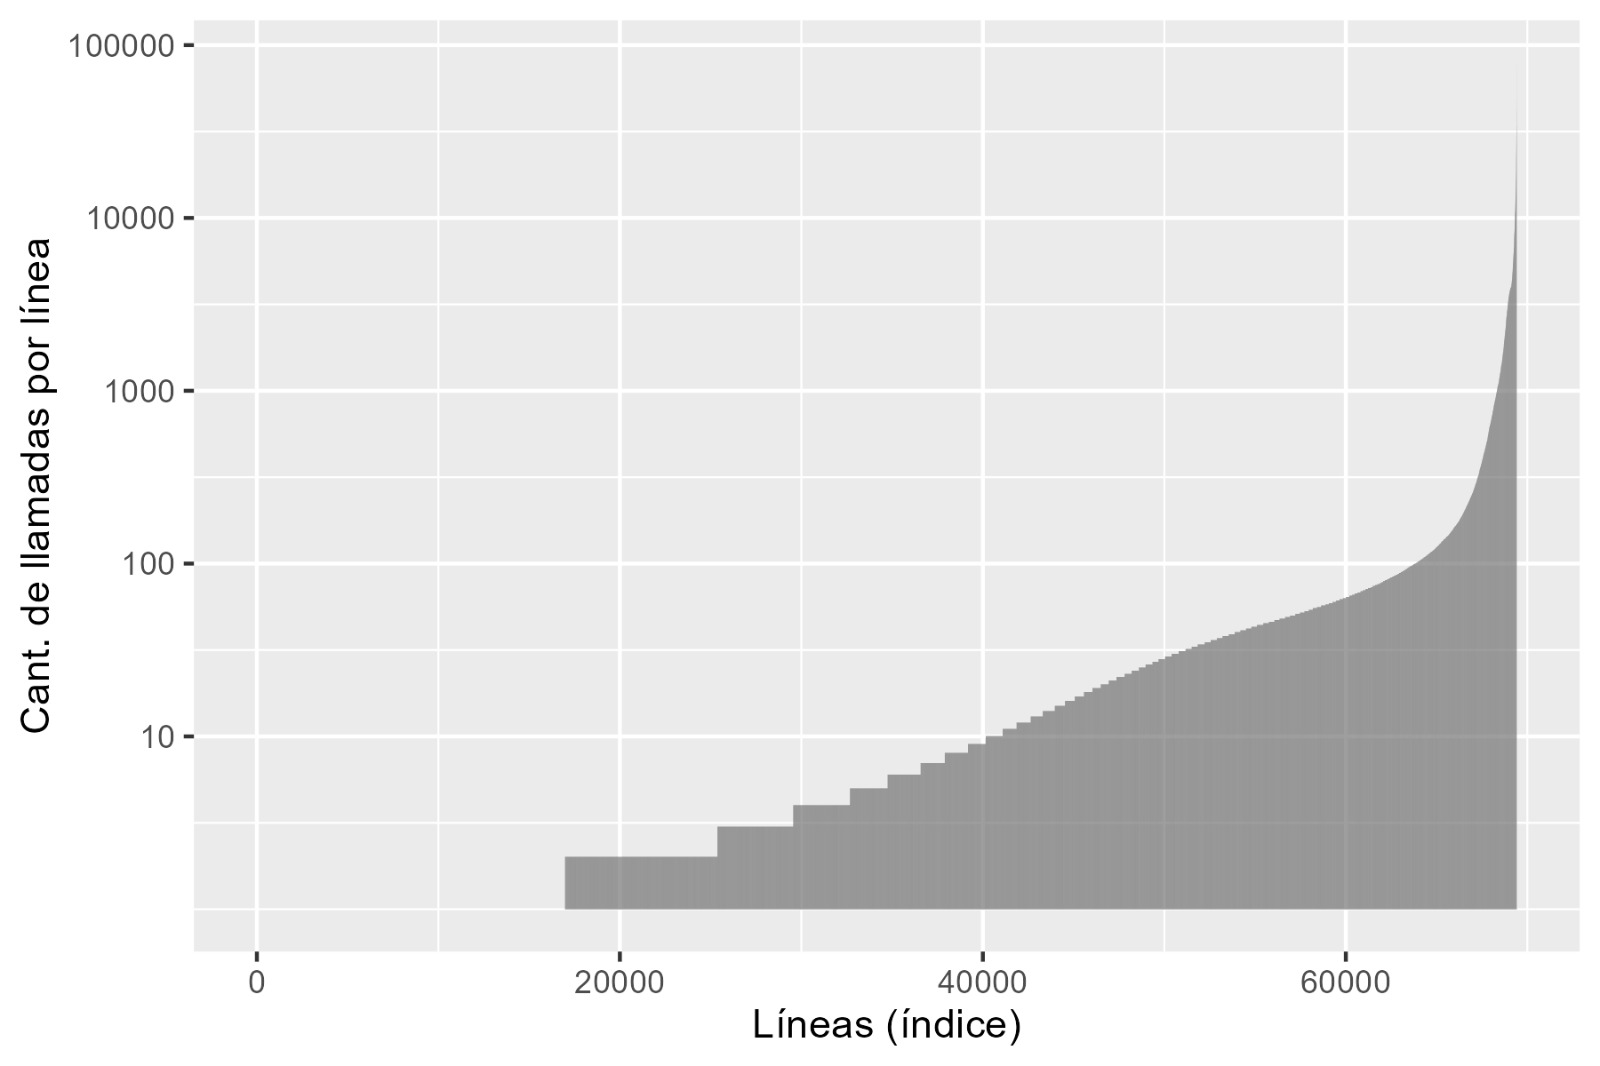
\includegraphics[width=\textwidth]{grafico_llamadas_01.jpeg}
		\caption{Distribución de comunicaciones salientes}
		\label{fig:enter-label}
	\end{figure}
	
	\section*{Determinación de las comunicaciones NO frecuentes}
	Considerando la distribución tan extrema de llamadas por dispositivos, se nos plantea el inconveniente de definir qué es un \textit{número NO frecuente}.\\
	En el caso de los salientes podemos hacer expresar esto con la siguiente tabla:\\
	
	\begin{table}[h]
		\centering
		\begin{tabular}{|c|c|}
			\hline
			Cantidad de dispositivos & Cantidad de llamadas\\
			\hline
			16979 & 1\\
			8396 & 2\\
			4178 & 3\\
			3127 & 4\\
			\hline
			32680 & 4 o menos\\
			\hline
			69414 & Todos\\
			\hline
		\end{tabular}
		\caption{Distribución comunicaciones salientes}
		\label{tab:t1}
	\end{table}
	Y en el caso de los entrantes
	\begin{table}[h]
		\centering
		\begin{tabular}{|c|c|}
			\hline
			Cantidad de dispositivos & Cantidad de llamadas\\
			\hline
			10443 & 1\\
			5111 & 2\\
			2761 & 3\\
			2143 & 4\\
			\hline
			18315 & 3 o menos\\
			\hline
			36828 & Todos\\
			\hline
		\end{tabular}
		\caption{Distribución comunicaciones entrantes}
		\label{tab:t2}
	\end{table}
	\\
	Podemos notar que en el caso de las comunicaciones salientes, si consideramos que los dispositivos NO frecuentes son los que realizaron 4 o menos llamadas, ya tenemos casi la mitad de los dispositivos registrados en las celdas consideradas.\\
	\\
	Y lo mismo ocurre con los dispositivos entrantes: considerando los dispositivos que recibieron 3 o menos comunicaciones ya tenemos mas de la mitad del total.\\
	\\
	Esto indica que hay pocos dispositivos que realizan o reciben una gran cantidad de comunicaciones y muchos dispositivos que se activan dentro de las celdas consideradas.\\
	Por lo tanto, es muy probable que los dispositivos de interés estén dentro de los que operan \textbf{1 o 2} comunicaciones dentro de las celdas.
	\section*{Comunicaciones NO frecuentes en las ventanas temporales}
	Eliminando los dispositivos no frecuentes dentro de la ventana de $\pm$ 20 minutos, podemos observar que se realizan 18 comunicaciones salientes y 17 entrantes.\\
	Y en la ventana de $\pm$ 5 minutos hay 5 salientes y 7 entrantes.\\
	\begin{table}[h]
		\centering
		\begin{tabular}{|c|c|c|c|c|}
			\hline
			Fecha y hora & Dispositivo & A donde &  Tipo comunicación & Duración (s)  \\
			\hline
			2023-09-07 20:26:33 & 1122747186 & 1156095002 & LLAM. LOCAL & 15\\
			2023-09-07 20:27:50 & 1168441770 & 1155812801 & LLAM. LOCAL & 25\\
			2023-09-07 20:29:03 & 1122363386 & 158759006 & Conexión Móvil & 336698679\\
			2023-09-07 20:29:14 & 1168310005 & 841310004 & Conexión Móvil & 10996\\
			2023-09-07 20:32:01 & 1134883024 & 2836713025 & Conexión Móvil & 26558134\\
			2023-09-07 20:32:34 & 1127975952 & 1309311007 & Conexión Móvil & 42925688\\
			2023-09-07 20:42:05 & 1131804484 & 348303885 & Tráfico incluido & 2130848\\
			2023-09-07 20:42:14 & 1131804484 & 348303886 & TRAFICO DATOS & 3997\\
			2023-09-07 20:44:12 & 1138863797 & 1964713016 & Conexión Móvil & 14236203\\
			2023-09-07 20:49:02 & 1157345937 & 2747 & ASIST.RET & 24\\
			2023-09-07 20:50:27 & 1137848153 & 2216611013 & Conexión Móvil & 122436479\\
			2023-09-07 20:51:10 & 1144751313 & 1153119614 & LLAM. LOCAL & 12\\
			2023-09-07 20:56:37 & 1162335309 & 159413025 & Conexion Movil & 9925536\\
			2023-09-07 21:00:22 & 1170286582 & 81469005 & Conexion Movil & 484\\
			2023-09-07 21:01:28 & 1161686108 & 1121684935 & LLAM. LOCAL & 82\\
			2023-09-07 21:02:31 & 1170286582 & 1909412029 & Conexion Movil & 188615353\\
			2023-09-07 21:03:29 & 1123488404 & 1137664349 & LLAM. LOCAL & 2\\
			2023-09-07 21:04:56 & 1132626386 & 2633212006 & Conexión Móvil & 4578116\\
			\hline
		\end{tabular}
		\caption{SALIENTES: Dispositivos no frecuentes en ventana de 20 minutos}
		\label{tab:t3}
	\end{table}
	\begin{table}[h]
		\centering
		\begin{tabular}{|c|c|c|c|c|}
			\hline
			Fecha y hora & Dispositivo & A donde &  Tipo comunicación & Duración (s)  \\
			\hline
			2023-09-07 20:42:05 & 1131804484 & 348303885 & Tráfico incluido & 2130848\\
			2023-09-07 20:42:14 & 1131804484 & 348303886 & TRAFICO DATOS & 3997\\
			2023-09-07 20:44:12 & 1138863797 & 1964713016 & Conexión Móvil & 14236203\\
			2023-09-07 20:49:02 & 1157345937 & 2747 & ASIST.RET & 24\\
			2023-09-07 20:50:27 & 1137848153 & 2216611013 & Conexión Móvil & 122436479\\
			\hline
		\end{tabular}
		\caption{SALIENTES: Dispositivos no frecuentes en ventana de 5 minutos}
		\label{tab:t4}
	\end{table}
	\begin{table}[h]
		\centering
		\begin{tabular}{|c|c|c|c|c|}
			\hline
			Fecha y hora & Dispositivo & Quien lo llamo & Duración (s)  \\
			\hline
			2023-09-07 20:25:08 & 1123841860 & 1150569808  & 48\\
			2023-09-07 20:31:39 & 1160363074 & 1169948365  & 57\\
			2023-09-07 20:33:08 & 1127224501 & 1165212800  & 65 \\
			2023-09-07 20:33:27 & 1155082345 & 1140633838  & 52   \\
			2023-09-07 20:34:28 & 1136542554 & 1126793382  & 24   \\
			2023-09-07 20:34:30 & 1136175661 & 1138700444  & 2   \\
			2023-09-07 20:40:55 & 1156294118 & 1164678323  & 365   \\
			2023-09-07 20:42:00 & 1133243077 & 1167686403  & 1   \\
			2023-09-07 20:42:29 & 1160191720 & 1169546648  & 43   \\
			2023-09-07 20:44:07 & 1160286644 & 1165654808  & 83   \\
			2023-09-07 20:47:38 & 1164165900 & 3813023189  & 5116   \\
			2023-09-07 20:48:45 & 1131910645 & 1158168696  & 148   \\
			2023-09-07 20:49:44 & 1157662720 & 1161190634  & 164   \\
			2023-09-07 20:52:42 & 1161234760 & 2234239322  & 7   \\
			2023-09-07 20:54:39 & 1132441220 & 1136313481  & 19   \\
			2023-09-07 20:57:39 & 1126860252 & 1170361319  & 71   \\
			2023-09-07 20:58:14 & 1139252329 & 1130921657  & 126   \\
			\hline
		\end{tabular}
		\caption{ENTRANTES: Dispositivos no frecuentes en ventana de 20 minutos}
		\label{tab:t5}
	\end{table}
	\begin{table}[h]
		\centering
		\begin{tabular}{|c|c|c|c|c|}
			\hline
			Fecha y hora & Dispositivo & Quien lo llamo & Duración (s)  \\
			\hline
			2023-09-07 20:40:55 & 1156294118 & 1164678323  & 365   \\
			2023-09-07 20:42:00 & 1133243077 & 1167686403  & 1   \\
			2023-09-07 20:42:29 & 1160191720 & 1169546648  & 43   \\
			2023-09-07 20:44:07 & 1160286644 & 1165654808  & 83   \\
			2023-09-07 20:47:38 & 1164165900 & 3813023189  & 5116   \\
			2023-09-07 20:48:45 & 1131910645 & 1158168696  & 148   \\
			2023-09-07 20:49:44 & 1157662720 & 1161190634  & 164   \\
			\hline
		\end{tabular}
		\caption{ENTRANTES: Dispositivos no frecuentes en ventana de 5 minutos}
		\label{tab:t5}
	\end{table}
	\clearpage
	\section*{Conclusión}
	A partir de la información suministrada por la compañía proveedora de servicios de telefonía celular, (haciendo notar que la información geográfica de las celdas no se corresponde con la de la zona del hecho) se procede a determinar qué números de dispositivo no son de operatoria frecuente en la zona.\\
	Obtenidos esos dispositivos, se comprueba cuáles de ellos fueron operados de forma saliente o entrante durante unas ventanas de tiempo alrededor de la hora del hecho.\\
	De esas comunicaciones se descartan las que son repetidas y las que son a un servicio de números cortos de la compañía celular (buzón de voz), llegándose a una lista de 32 identificadores de dispositivo que serían de interés.\\
	
	Los números  de interés son:
	\begin{itemize}
		\item \textcolor{red}{1157662720}
		\item 1132441220
		\item \textcolor{red}{1164165900}
		\item 1127975952
		\item 1123488404
		\item 1168441770
		\item 1136175661
		\item 1122747186
		\item \textcolor{red}{1160286644}
		\item \textcolor{red}{1138863797}
		\item 1127224501
		\item 1160363074
		\item \textcolor{red}{1131804484}
		\item 1123841860
		\item \textcolor{red}{1133243077}
		\item 1161234760
		\item 1162335309
		\item 1134883024
		\item 1144751313
		\item 1132626386
		\item \textcolor{red}{1137848153}
		\item 1136542554
		\item 1161686108
		\item 1126860252
		\item \textcolor{red}{1156294118}
		\item \textcolor{red}{1160191720}
		\item 1155082345
		\item 1139252329
		\item 1168310005
		\item 1170286582
		\item \textcolor{red}{1131910645}
		\item 1122363386
	\end{itemize}
	
	Los números en rojo son los correspondientes a la ventana de $\pm$ 5 minutos.
\end{document}